\chapter{Implementation}

We created a web app in order to benchmark our work.

As this was part of our access management platform and requirement for our project, we implemented this floorplan also in our web application.

\begin{figure}[!hb]
	\centering
	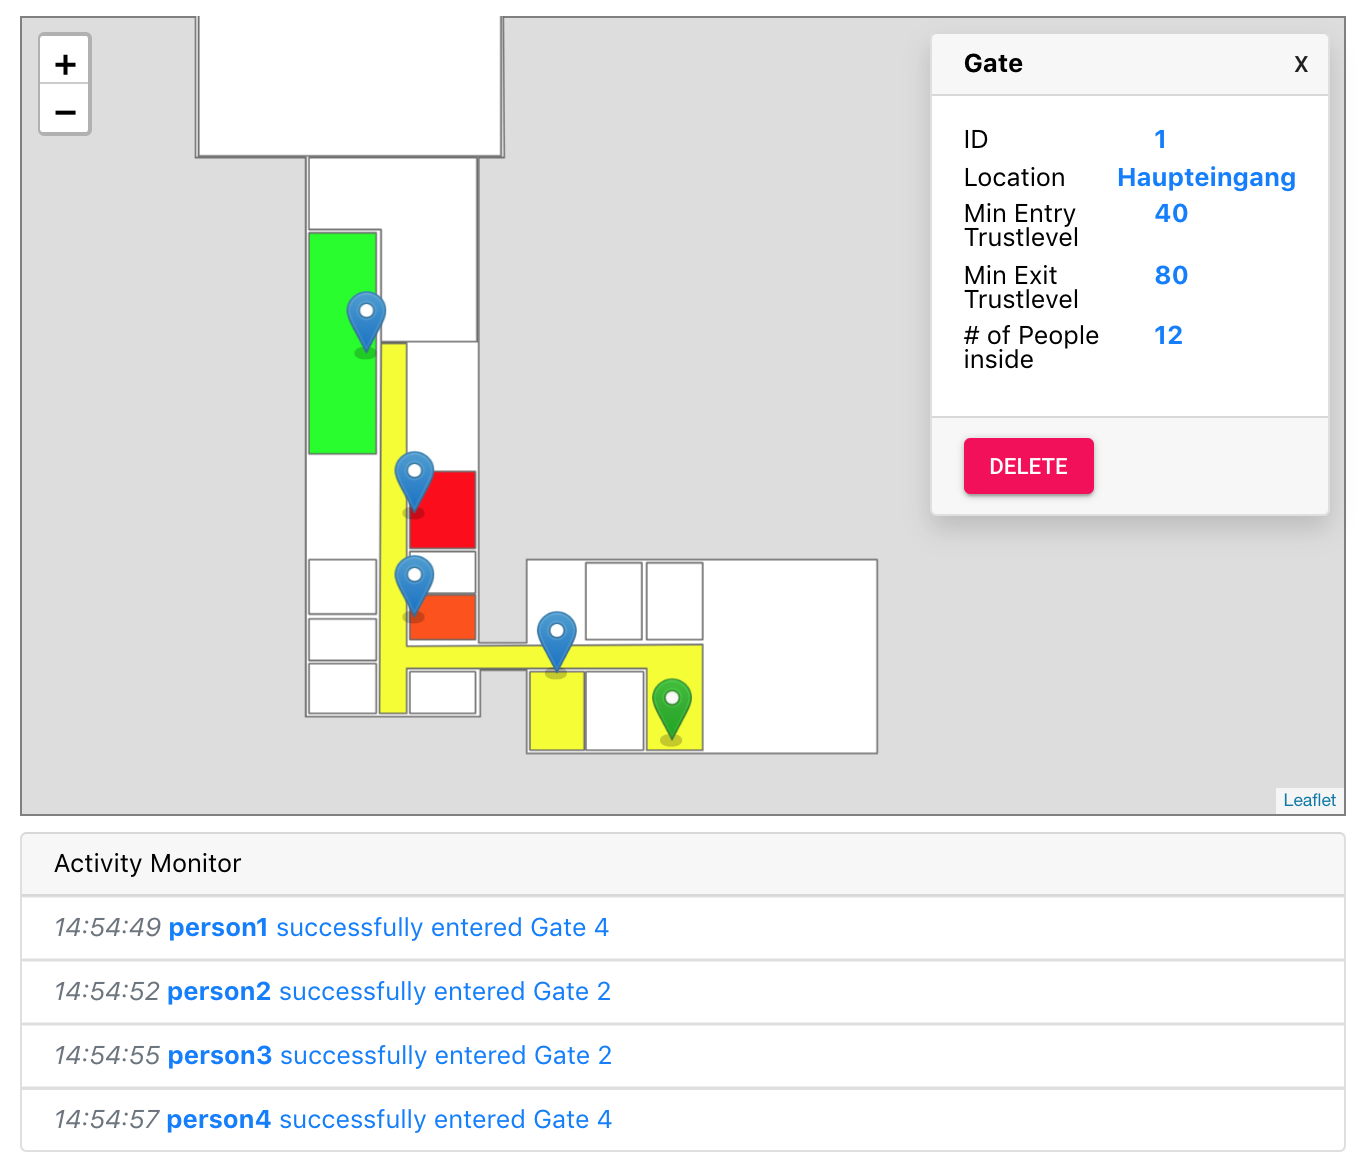
\includegraphics[width=0.9\linewidth]{images/FloorplanScreenshot}
	\caption{Screenshot of the implemented interactive floorplan}
	\label{fig:FloorplanScreenshot}
\end{figure}

\section{Display of Indoor features}
\label{Display of Indoor features}

\section{Logging of Gate Events}
\label{Logging of Gate Events}

\section{Real-time Floorplan}
\label{Real-time Floorplan}

Socket io server side

Socket io client side

\begin{lstlisting}[label=socketIOClientSide]
listenForGateEvents = () => {
        const socket = io({
            secure: true,
            transport: ['websocket'],
            query: {
                token: sessionStorage.getItem('kctoken'),
            },
            jsonp: false,
        });

        socket.on('gateEvent', (event) => { this.gateEventHappened(event); });
        socket.on('gateAlarm', (event) => { this.gateAlarmHappened(event); });
    };
\end{lstlisting}

\subsection{Access Decision Information}

\subsection{Heatmap}

\section{Persisting Data}
\label{Persisting Data}


Security (Hard Coded Token)

